\documentclass[11pt]{article}
\usepackage[textwidth=18.0cm, textheight=23.0cm, top=2.0cm]{geometry}
\usepackage{pst-all}
\usepackage{amssymb}
\usepackage{tikz}
\usepackage{underscore}\begin{document}
\pagestyle{empty}


ClassName: \underline{\textbf{Class_07.2bp-9}}
\par
BinSize: \underline{\textbf{100 × 100}}
\par
ReduceSize: \underline{\textbf{100 × 100}}
\par
TypeNum: \underline{\textbf{19}}
\par
Num: \underline{\textbf{20}}
\par
OutS: \underline{\textbf{40000}}
\par
InS: \underline{\textbf{34213}}
\par
Rate: \underline{\textbf{0.855}}
\par
UB: \underline{\textbf{4}}
\par
LB0: \underline{\textbf{4}}
\par
LB: \underline{\textbf{4}}
\par
LBWithCut: \underline{\textbf{4}}
\par
NodeCut: \underline{\textbf{0}}
\par
ExtendedNodeCnt: \underline{\textbf{1}}
\par
GenNodeCnt: \underline{\textbf{1}}
\par
PrimalNode: \underline{\textbf{0}}
\par
ColumnCount: \underline{\textbf{4}}
\par
TotalCutCount: \underline{\textbf{0}}
\par
RootCutCount: \underline{\textbf{0}}
\par
LPSolverCnt: \underline{\textbf{1}}
\par
PricingSolverCnt: \underline{\textbf{0}}
\par
BranchAndBoundNum: \underline{\textbf{1}}
\par
isOpt: \underline{\textbf{true}}
\par
TimeOnPrimal: \underline{\textbf{0.000 s}}
\par
TimeOnPricing: \underline{\textbf{0.000 s}}
\par
TimeOnRmp: \underline{\textbf{0.063 s}}
\par
TotalTime: \underline{\textbf{0.125 s}}
\par
\newpage


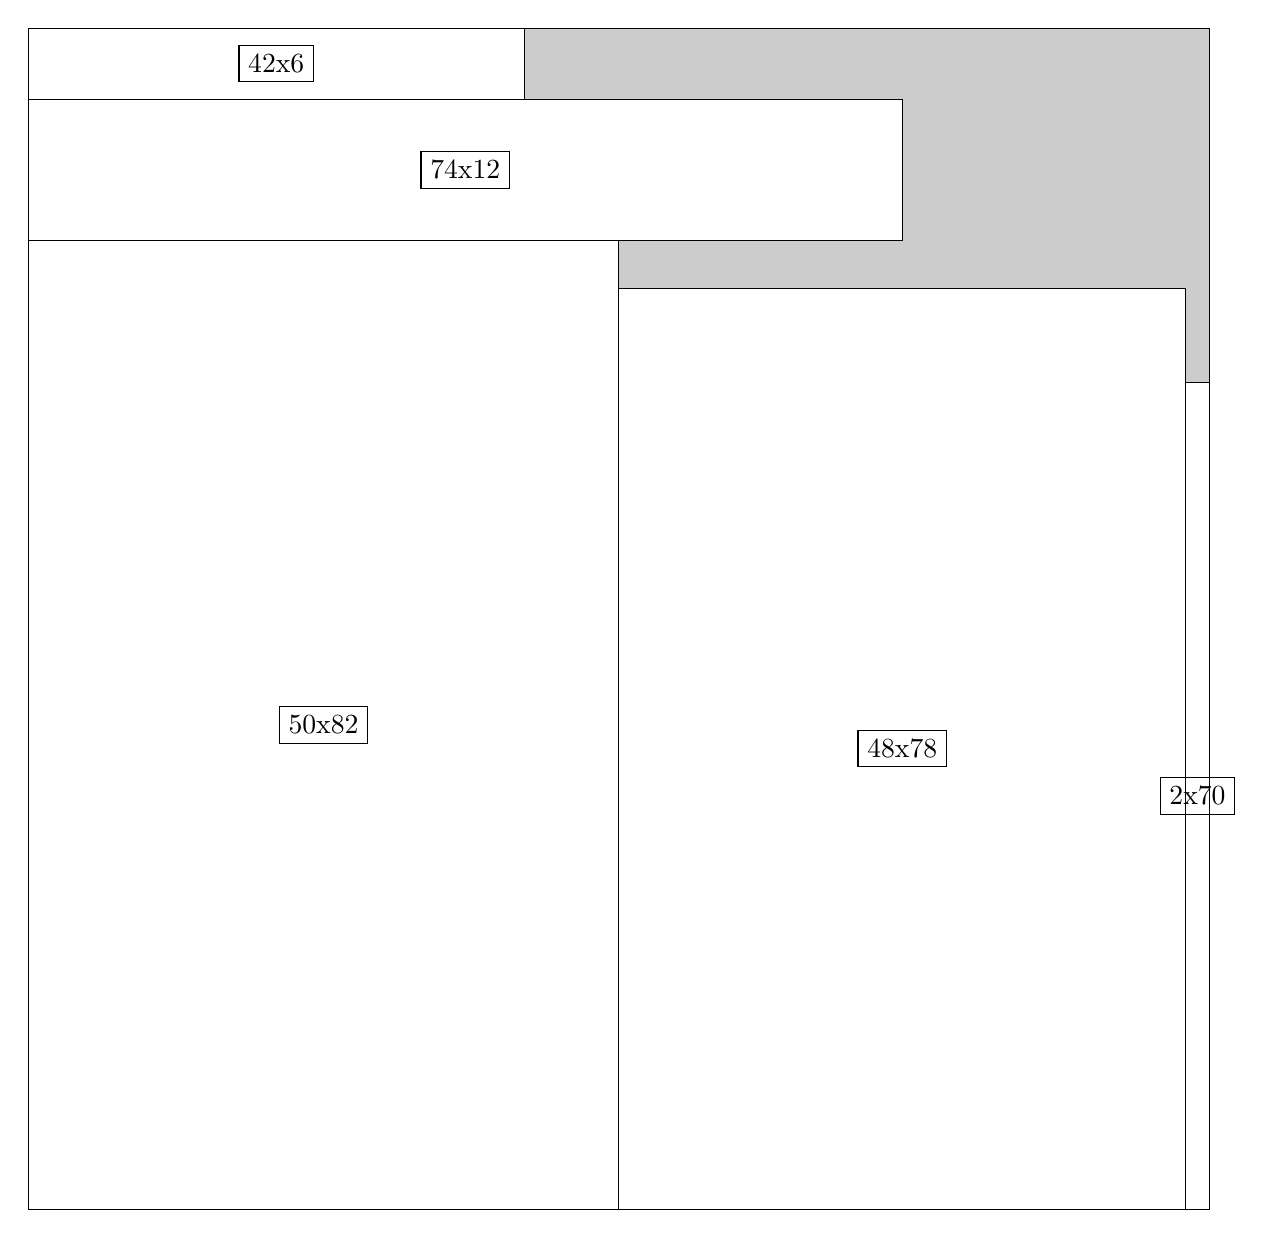
\begin{tikzpicture}[shorten >=1pt,scale=1.0,every node/.style={scale=1.0},->]
\tikzstyle{vertex}=[circle,fill=black!25,minimum size=14pt,inner sep=0pt]
\filldraw[fill=gray!40!white, draw=black] (0,0) rectangle (15.0,15.0);
\foreach \name/\x/\y/\w/\h in {50x82/0.0/0.0/7.5/12.299999999999999,48x78/7.5/0.0/7.199999999999999/11.7,74x12/0.0/12.299999999999999/11.1/1.7999999999999998,42x6/0.0/14.1/6.3/0.8999999999999999,2x70/14.7/0.0/0.3/10.5}
\filldraw[fill=white!40!white, draw=black] (\x,\y) rectangle node[draw] (\name) {\name} ++(\w,\h);
\end{tikzpicture}


w =50 , h =82 , x =0 , y =0 , v =4100
\par
w =48 , h =78 , x =50 , y =0 , v =3744
\par
w =74 , h =12 , x =0 , y =82 , v =888
\par
w =42 , h =6 , x =0 , y =94 , v =252
\par
w =2 , h =70 , x =98 , y =0 , v =140
\par
\newpage


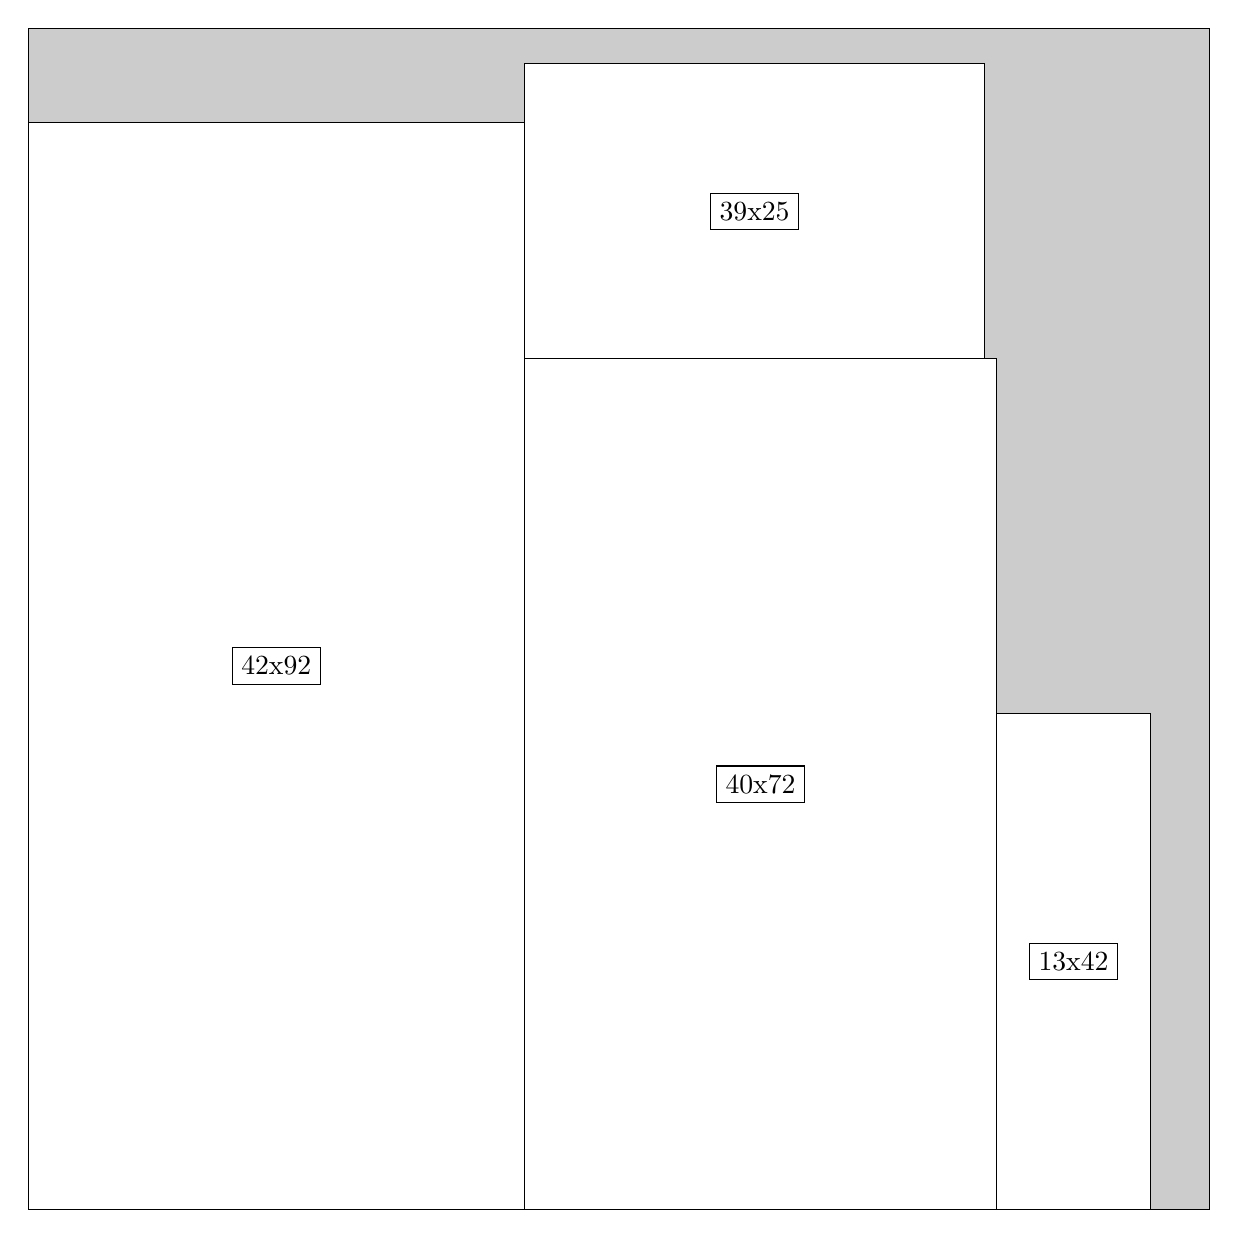
\begin{tikzpicture}[shorten >=1pt,scale=1.0,every node/.style={scale=1.0},->]
\tikzstyle{vertex}=[circle,fill=black!25,minimum size=14pt,inner sep=0pt]
\filldraw[fill=gray!40!white, draw=black] (0,0) rectangle (15.0,15.0);
\foreach \name/\x/\y/\w/\h in {42x92/0.0/0.0/6.3/13.799999999999999,40x72/6.3/0.0/6.0/10.799999999999999,39x25/6.3/10.799999999999999/5.85/3.75,13x42/12.299999999999999/0.0/1.95/6.3}
\filldraw[fill=white!40!white, draw=black] (\x,\y) rectangle node[draw] (\name) {\name} ++(\w,\h);
\end{tikzpicture}


w =42 , h =92 , x =0 , y =0 , v =3864
\par
w =40 , h =72 , x =42 , y =0 , v =2880
\par
w =39 , h =25 , x =42 , y =72 , v =975
\par
w =13 , h =42 , x =82 , y =0 , v =546
\par
\newpage


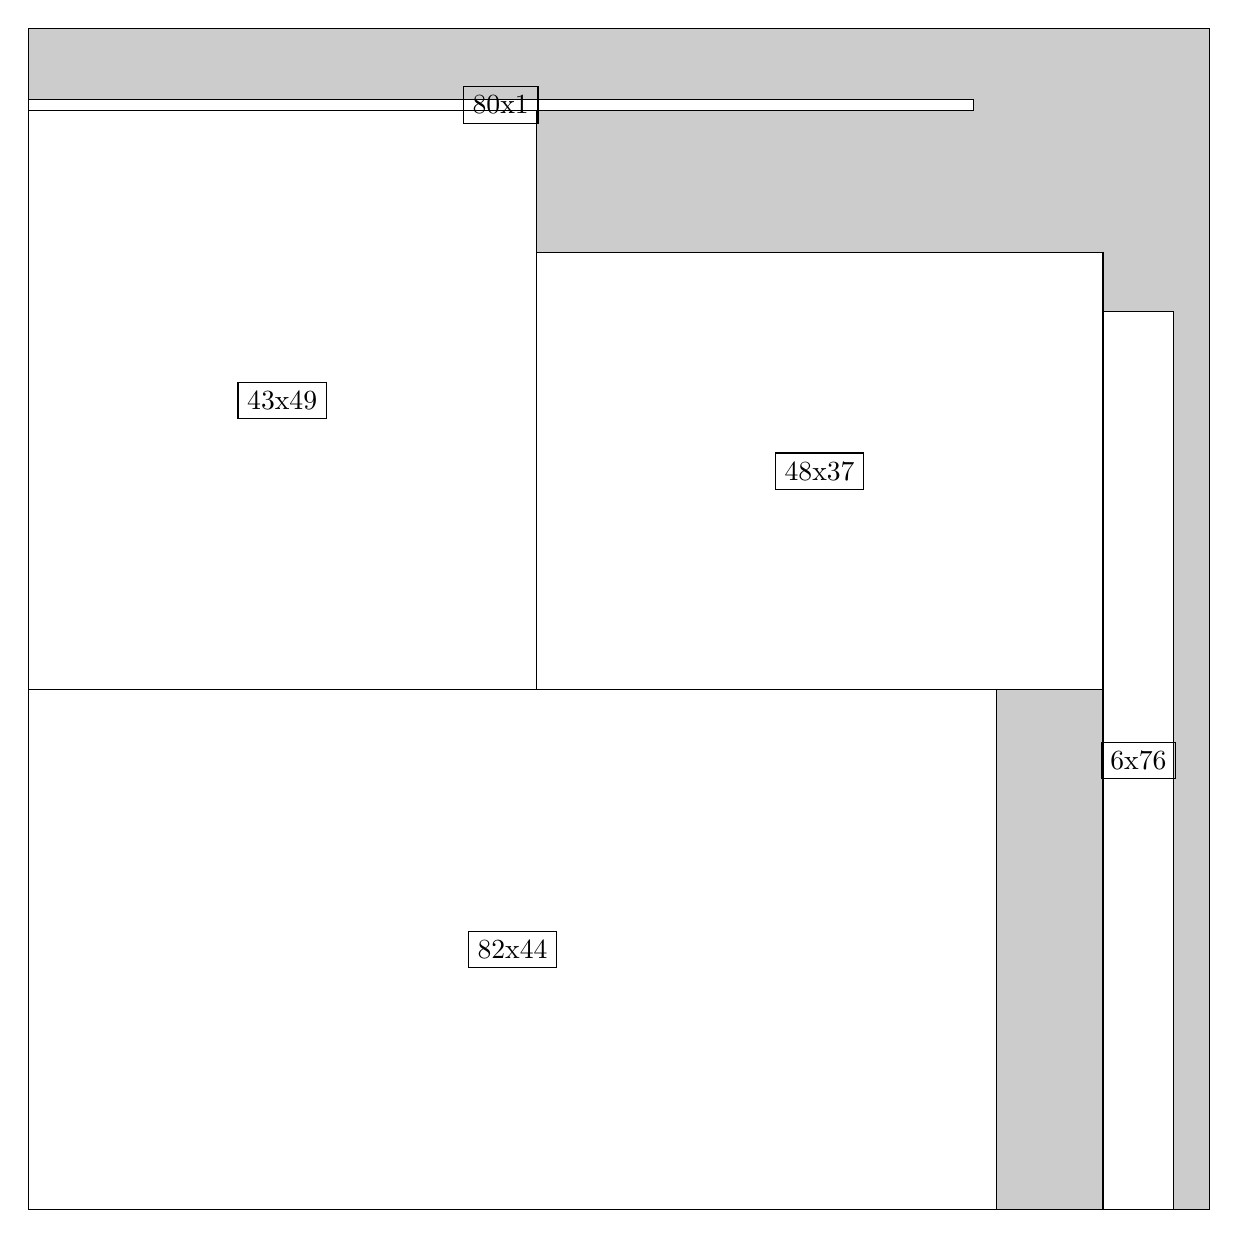
\begin{tikzpicture}[shorten >=1pt,scale=1.0,every node/.style={scale=1.0},->]
\tikzstyle{vertex}=[circle,fill=black!25,minimum size=14pt,inner sep=0pt]
\filldraw[fill=gray!40!white, draw=black] (0,0) rectangle (15.0,15.0);
\foreach \name/\x/\y/\w/\h in {82x44/0.0/0.0/12.299999999999999/6.6,43x49/0.0/6.6/6.45/7.35,48x37/6.45/6.6/7.199999999999999/5.55,6x76/13.65/0.0/0.8999999999999999/11.4,80x1/0.0/13.95/12.0/0.15}
\filldraw[fill=white!40!white, draw=black] (\x,\y) rectangle node[draw] (\name) {\name} ++(\w,\h);
\end{tikzpicture}


w =82 , h =44 , x =0 , y =0 , v =3608
\par
w =43 , h =49 , x =0 , y =44 , v =2107
\par
w =48 , h =37 , x =43 , y =44 , v =1776
\par
w =6 , h =76 , x =91 , y =0 , v =456
\par
w =80 , h =1 , x =0 , y =93 , v =80
\par
\newpage


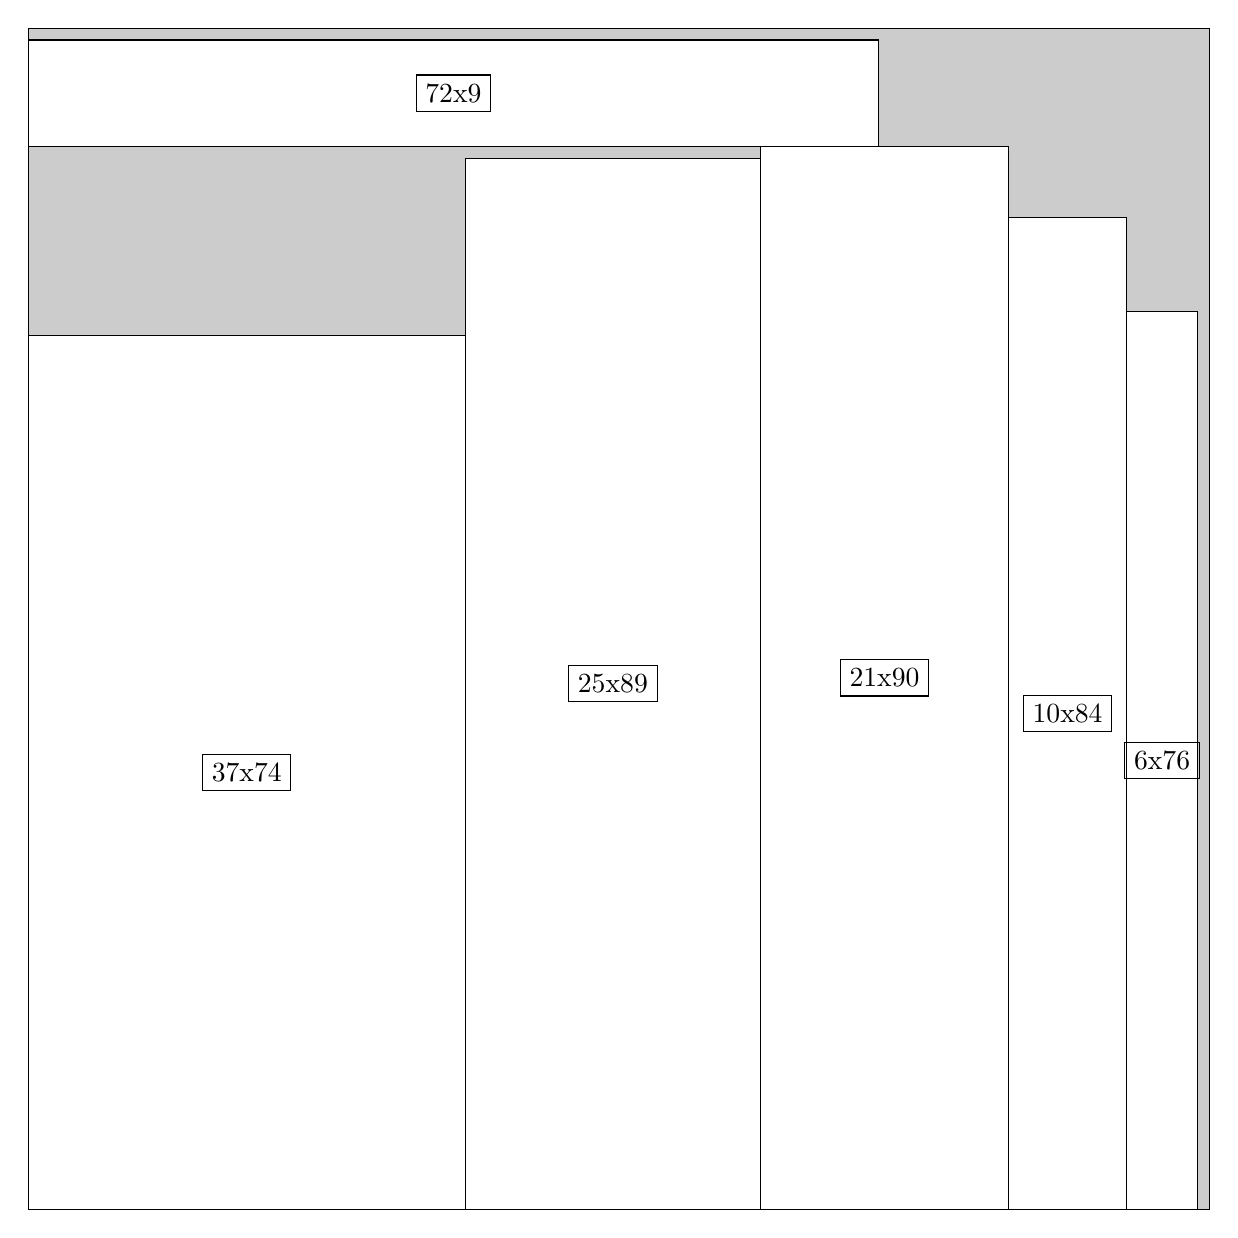
\begin{tikzpicture}[shorten >=1pt,scale=1.0,every node/.style={scale=1.0},->]
\tikzstyle{vertex}=[circle,fill=black!25,minimum size=14pt,inner sep=0pt]
\filldraw[fill=gray!40!white, draw=black] (0,0) rectangle (15.0,15.0);
\foreach \name/\x/\y/\w/\h in {37x74/0.0/0.0/5.55/11.1,25x89/5.55/0.0/3.75/13.35,21x90/9.299999999999999/0.0/3.15/13.5,10x84/12.45/0.0/1.5/12.6,72x9/0.0/13.5/10.799999999999999/1.3499999999999999,6x76/13.95/0.0/0.8999999999999999/11.4}
\filldraw[fill=white!40!white, draw=black] (\x,\y) rectangle node[draw] (\name) {\name} ++(\w,\h);
\end{tikzpicture}


w =37 , h =74 , x =0 , y =0 , v =2738
\par
w =25 , h =89 , x =37 , y =0 , v =2225
\par
w =21 , h =90 , x =62 , y =0 , v =1890
\par
w =10 , h =84 , x =83 , y =0 , v =840
\par
w =72 , h =9 , x =0 , y =90 , v =648
\par
w =6 , h =76 , x =93 , y =0 , v =456
\par
\newpage


\end{document}